\documentclass[a4paper, 10pt]{article}
\usepackage{scrextend}
\changefontsizes{9pt}
\usepackage{colortbl}
% Per-subject config for this repo. See vendor/template/course-config.tex.example
% for what each macro is used for.

\newcommand{\CourseCode}{2110473}
\newcommand{\CourseName}{Fault Tolerant Computing}
\newcommand{\StudentID}{6733172621}
\newcommand{\StudentName}{Patthadon Phengpinij}
\newcommand{\DefaultCollaborators}{Claude (for\,\LaTeX\,styling and grammar checking)}
\newcommand{\AssignmentLabel}{Homework}

\usepackage{../vendor/template/CEDT-Assignment-style}


\begin{document}
\subject
\asgntitle{10}{}{Week 12}{\StudentID\ \StudentName}{\DefaultCollaborators}

% ================================================================================ %
\section{Sequential Circuit Testing}
% ================================================================================ %

% ================================================================================ %
%                                    Problem 01                                    %
% ================================================================================ %
\begin{problem}
Find a checking sequence of this state table using the successor tree.

\myspace

% State table (left) and successor tree (right), side by side
\begin{table}[htbp]
\centering
\begin{minipage}[c]{0.48\linewidth}
    \centering

    % Colors
    \definecolor{titleblue}{RGB}{80,135,190}
    \definecolor{headerblue}{RGB}{207,217,232}
    \definecolor{rowlight}{RGB}{233,238,246}

    \renewcommand{\arraystretch}{1.5}
    \setlength{\tabcolsep}{10pt}

    \begin{tabular}{|c|c|c|}
        \hline
        \rowcolor{titleblue}
        \multicolumn{3}{|c|}{
            \color{white}\bfseries State Table
        } \\
        \hline

        \rowcolor{headerblue}
        & \multicolumn{2}{c|}{\bfseries Input} \\
        \arrayrulecolor{headerblue}\cline{1-1}\arrayrulecolor{black}\cline{2-3}
        \noalign{\vskip\arrayrulewidth} % keep the rule from being painted over by the next row's fill

        \rowcolor{headerblue}
        \multirow{-2}{*}{\bfseries\shortstack{Present\\State}}
        & $X=0$ & $X=1$ \\
        \hline

        \rowcolor{white}
        A & B,1 & C,0 \\
        \hline

        \rowcolor{rowlight}
        B & A,0 & D,1 \\
        \hline

        \rowcolor{white}
        C & B,0 & A,0 \\
        \hline

        \rowcolor{rowlight}
        D & C,1 & A,1 \\
        \hline
    \end{tabular}

    \caption{State transition and output table}
    \label{tab:state-table}
\end{minipage}%
\hfill
\begin{minipage}[c]{0.48\linewidth}
\centering
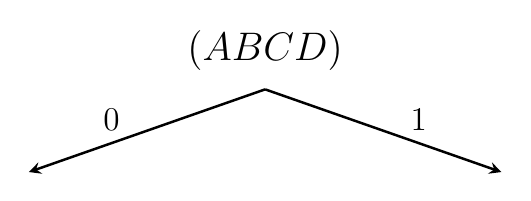
\begin{tikzpicture}[
    >=stealth,
    edge/.style={
        draw=black,
        line width=0.9pt,
        ->,
        >=stealth
    },
    state/.style={
        font=\Large,
        inner sep=1pt
    },
    branchlabel/.style={
        font=\large,
        inner sep=2pt
    }
]

% =========================================================
% Root and child coordinates
% =========================================================

\coordinate (root) at (0,0);

\coordinate (leftchild) at (-3.0,-1.05);
\coordinate (rightchild) at (3.0,-1.05);

% =========================================================
% Root state
% =========================================================

\node[state,above=0.20cm] at (root)
    {$(ABCD)$};

% =========================================================
% Successor branches
% =========================================================

% Input X = 0
\draw[edge]
    (root) -- (leftchild)
    node[
        branchlabel,
        pos=0.65,
        above=2pt
    ] {$0$};

% Input X = 1
\draw[edge]
    (root) -- (rightchild)
    node[
        branchlabel,
        pos=0.65,
        above=2pt
    ] {$1$};

% =========================================================
% Optional successor state labels
% =========================================================

% \node[state,below] at (leftchild) {$(BABC)$};
% \node[state,below] at (rightchild) {$(CDAA)$};

\end{tikzpicture}
\end{minipage}%
\end{table}

\end{problem}

\begin{solution}
	\noindent\textbf{Successor tree} (each node groups the states that are still indistinguishable, by output):
	\begin{center}
		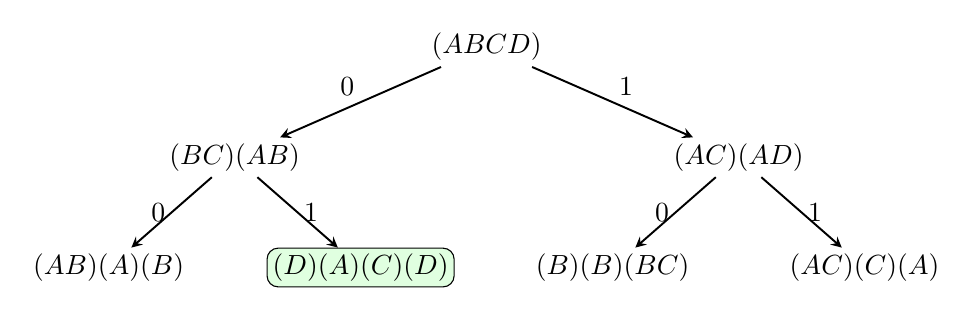
\begin{tikzpicture}[
				>=stealth, every node/.style={inner sep=2pt},
				edge/.style={draw, ->, line width=0.7pt},
				lvl/.style={font=\small}
			]
			\node (r)   at (0,0)      {$(ABCD)$};
			\node (n0)  at (-3.2,-1.4) {$(BC)(AB)$};
			\node (n1)  at (3.2,-1.4)  {$(AC)(AD)$};
			\node (n00) at (-4.8,-2.8) {$(AB)(A)(B)$};
			\node[draw, rounded corners, fill=green!12] (n01) at (-1.6,-2.8) {$(D)(A)(C)(D)$};
			\node (n10) at (1.6,-2.8)  {$(B)(B)(BC)$};
			\node (n11) at (4.8,-2.8)  {$(AC)(C)(A)$};
			\draw[edge] (r) -- node[above left]  {0} (n0);
			\draw[edge] (r) -- node[above right] {1} (n1);
			\draw[edge] (n0) -- node[left]  {0} (n00);
			\draw[edge] (n0) -- node[right] {1} (n01);
			\draw[edge] (n1) -- node[left]  {0} (n10);
			\draw[edge] (n1) -- node[right] {1} (n11);
		\end{tikzpicture}
	\end{center}
	The node reached by \(01\) contains only singletons, so \(X = 01\) is a distinguishing sequence:
	\begin{center}
		\begin{tabular}{c|cccc}
			\toprule
			Initial state         & A & B & C & D \\
			\midrule
			Response to \(X=01\)  & 11 & 00 & 01 & 10 \\
			Final state           & D & C & D & A \\
			\bottomrule
		\end{tabular}
	\end{center}
	\(110\) is a synchronizing sequence (every state goes to \(B\)), so it is used to initialize the machine.

	\noindent\textbf{Checking sequence} (\(X = 01\)):
	\begin{center}
		\setlength{\tabcolsep}{4pt}
		\begin{tabular}{l|l|c|c|c}
			\toprule
			Part & Purpose & Input & Output & End state \\
			\midrule
			Initialize & synchronize to \(B\) & 110 & -- & B \\
			\midrule
			Identify states & \(B\xrightarrow{X}C\xrightarrow{X}D\xrightarrow{X}A\xrightarrow{X}D\xrightarrow{X}A\) & 01\,01\,01\,01\,01 & 00\,01\,10\,11\,10 & A \\
			\midrule
			\multirow{11}{*}{Check transitions}
			 & \(A\xrightarrow{0/1}B\) & 0\,01 & 1\,00 & C \\
			 & \(C\xrightarrow{0/0}B\) & 0\,01 & 0\,00 & C \\
			 & \(C\xrightarrow{1/0}A\) & 1\,01 & 0\,11 & D \\
			 & \(D\xrightarrow{0/1}C\) & 0\,01 & 1\,01 & D \\
			 & \(D\xrightarrow{1/1}A\) & 1\,01 & 1\,11 & D \\
			 & transfer \(D\to A\)     & 01    & 10    & A \\
			 & \(A\xrightarrow{1/0}C\) & 1\,01 & 0\,01 & D \\
			 & transfer \(D\to B\)     & 00    & 10    & B \\
			 & \(B\xrightarrow{0/0}A\) & 0\,01 & 0\,11 & D \\
			 & transfer \(D\to B\)     & 00    & 10    & B \\
			 & \(B\xrightarrow{1/1}D\) & 1\,01 & 1\,10 & A \\
			\bottomrule
		\end{tabular}
	\end{center}
	\[
		\boxed{\text{Input: } 110\;0101010101\;001\,001\,101\,001\,101\,01\,101\,00\,001\,00\,101}
	\]
	\[
		\text{Expected output (after initialization): } 0001101110\;100\,000\,011\,101\,111\,10\,001\,10\,011\,10\,110
	\]
\end{solution}
% ================================================================================ %

% ================================================================================ %
%                                    Problem 02                                    %
% ================================================================================ %
\begin{problem}
Find the test sequence for \( s-a-1 \) on line \( u \).

\myspace

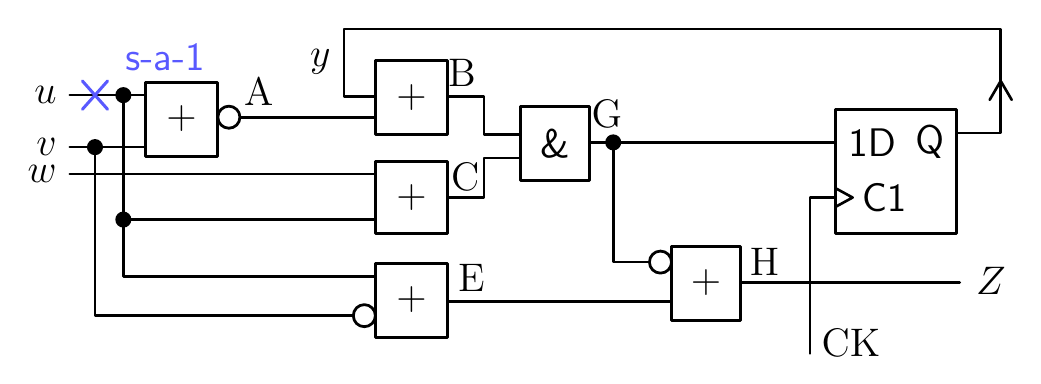
\begin{tikzpicture}[
    x=0.020cm, y=-0.020cm,
    wire/.style={
        draw=black,
        line width=0.95pt,
        line cap=round,
        line join=round
    },
    gate/.style={
        draw=black,
        fill=white,
        line width=1.0pt,
        line cap=round,
        line join=round
    },
    inputlabel/.style={
        font=\Large,
        inner sep=0pt
    },
    outputlabel/.style={
        font=\Large,
        inner sep=0pt
    },
    signallabel/.style={
        font=\Large,
        inner sep=0pt
    },
    gatetext/.style={
        font=\sffamily\Large,
        inner sep=0pt
    },
    fault/.style={
        draw=blue!65,
        line width=1.1pt,
        line cap=round
    }
]

% =========================================================
% Input wires: u, v, w
% =========================================================

\draw[wire] (61,85) -- (109,85);
\draw[wire] (61,118) -- (109,118);
\draw[wire] (61,135) -- (255,135);

% =========================================================
% Input branching
% =========================================================

% u -> C and E
\draw[wire]
    (95,85) -- (95,200) -- (255,200);

\draw[wire]
    (95,164) -- (255,164);

% v -> inverted input of E
\draw[wire]
    (77,118) -- (77,225) -- (242,225);

% =========================================================
% Gate A output -> B
% =========================================================

\draw[wire]
    (169,99) -- (255,99);

% =========================================================
% B and C outputs -> G
% =========================================================

% B -> upper input of G
\draw[wire]
    (301,86) -- (324,86)
    -- (324,110) -- (347,110);

% C -> lower input of G
\draw[wire]
    (301,150) -- (324,150)
    -- (324,125) -- (347,125);

% =========================================================
% G output -> D flip-flop and H
% =========================================================

% G -> D input
\draw[wire]
    (391,115) -- (547,115);

% G -> inverted upper input of H
\draw[wire]
    (406,115) -- (406,191) -- (429,191);

% =========================================================
% E output -> H
% =========================================================

\draw[wire]
    (301,216) -- (443,216);

% =========================================================
% H output -> Z
% =========================================================

\draw[wire]
    (487,204) -- (626,204);

% =========================================================
% Clock input
% =========================================================

\draw[wire]
    (531,249) -- (531,150) -- (547,150);

% =========================================================
% Flip-flop output and feedback loop
% =========================================================

\draw[wire]
    (624,109) -- (652,109)
    -- (652,43) -- (235,43)
    -- (235,86) -- (255,86);

% Feedback direction arrow (upward)
\draw[wire]
    (645,88) -- (652,76) -- (659,88);

% =========================================================
% Gate A : NOT-output block
% =========================================================

\draw[gate]
    (109,77) rectangle (155,124);

% Output inversion bubble
\draw[gate]
    (162,99) circle[radius=7];

% =========================================================
% Gate B : + block
% =========================================================

\draw[gate]
    (255,63) rectangle (301,110);

% =========================================================
% Gate C : + block
% =========================================================

\draw[gate]
    (255,127) rectangle (301,173);

% =========================================================
% Gate E : + block
% =========================================================

\draw[gate]
    (255,192) rectangle (301,239);

% Lower input inversion bubble
\draw[gate]
    (248,225) circle[radius=7];

% =========================================================
% Gate G : AND block
% =========================================================

\draw[gate]
    (347,92) rectangle (391,139);

% =========================================================
% Gate H : + block
% =========================================================

\draw[gate]
    (443,181) rectangle (487,228);

% Upper input inversion bubble
\draw[gate]
    (436,191) circle[radius=7];

% =========================================================
% D Flip-Flop
% =========================================================

% Flip-flop body
\draw[gate]
    (547,94) rectangle (624,173);

% Clock trigger symbol
\draw[wire]
    (547,144) -- (558,150) -- (547,156);

% =========================================================
% Junction dots
% =========================================================

\foreach \p in {
    (95,85),
    (77,118),
    (95,164),
    (406,115)
}{
    \fill[black] \p circle[radius=5.1];
}

% =========================================================
% Gate symbols
% =========================================================

\node[gatetext] at (132,100) {$+$};
\node[gatetext] at (278,86.5) {$+$};
\node[gatetext] at (278,150) {$+$};
\node[gatetext] at (278,215) {$+$};

\node[gatetext] at (369,116) {\&};
\node[gatetext] at (465,204) {$+$};

% =========================================================
% D Flip-Flop labels
% =========================================================

\node[gatetext,anchor=west]
    at (555,115) {1D};

\node[gatetext]
    at (607,115) {Q};

\node[gatetext]
    at (578,150) {C1};

% =========================================================
% External input/output labels
% =========================================================

\node[inputlabel,anchor=east]
    at (53,85) {$u$};

\node[inputlabel,anchor=east]
    at (53,118) {$v$};

\node[inputlabel,anchor=east]
    at (53,135) {$w$};

\node[outputlabel,anchor=west]
    at (636,203) {$Z$};

\node[signallabel,anchor=west]
    at (538,242) {CK};

% =========================================================
% Internal signal labels
% =========================================================

\node[signallabel] at (181,83) {A};
\node[signallabel] at (310,71) {B};
\node[signallabel] at (312,137) {C};
\node[signallabel] at (316,201) {E};
\node[signallabel] at (402,97) {G};
\node[signallabel] at (502,191) {H};

% Feedback signal label
\node[signallabel] at (220,64) {$y$};

% =========================================================
% Stuck-at-1 fault annotation
% =========================================================

% Blue X on wire u
\draw[fault] (69,76) -- (85,94);
\draw[fault] (69,94) -- (85,76);

% Fault label
\node[
    font=\sffamily\Large,
    text=blue!65,
    anchor=south west,
    inner sep=0pt
] at (96,70) {s-a-1};

\end{tikzpicture}

\end{problem}

\begin{solution}
	\noindent Circuit equations (\(y\) = flip-flop output, \(Y\) = next state):
	\[
		A = \overline{u+v},\quad B = y + A,\quad C = u + w,\quad E = u + \overline{v},\quad
		G = BC,\quad Z = H = \overline{G} + E,\quad Y = G.
	\]
	\noindent\textbf{Faulty machine} (\(u = 1\)): \(E = 1 \Rightarrow Z = 1\) for every input and state.

	\myspace
	
	\noindent\textbf{Good machine:} we need \(Z = 0\), i.e.\ \(u = 0\), \(v = 1\), \(G = 1\).
	With \(u = 0, v = 1\): \(A = 0\), so \(G = y\,w\), requiring \(y = 1\) and \(w = 1\).
	Since the initial state is unknown, \(y = 1\) must be set first:
	with \(u = 0, v = 0\), \(A = 1 \Rightarrow G = w\), so \(w = 1\) gives \(Y = 1\) for any \(y\).
	\begin{center}
		\begin{tabular}{c|ccc|c|cccccc|c|c}
			\toprule
			Time & \(u\) & \(v\) & \(w\) & \(y\) & \(A\) & \(B\) & \(C\) & \(E\) & \(G\) & \(Y\) & \(Z\) & \(Z_{\text{faulty}}\) \\
			\midrule
			1 & 0 & 0 & 1 & \(x\) & 1 & 1 & 1 & 1 & 1 & 1 & 1 & 1 \\
			2 & 0 & 1 & 1 & 1     & 0 & 1 & 1 & 0 & 1 & 1 & \textbf{0} & \textbf{1} \\
			\bottomrule
		\end{tabular}
	\end{center}
	\[ \boxed{(u\,v\,w) = 001,\ 011} \]
	The fault is detected at time 2 (\(Z = 0\) good, \(Z = 1\) faulty).
\end{solution}
% ================================================================================ %

\end{document}
